\chapter{乱流の統計的普遍則と動力学}
\label{chap:StatisticalUniversalityAndDynamicsOfTurbulence}
% prefix: SUADOT

本章では,今日の乱流理論の基礎となっているKolmogorovの理論を,局所平衡仮説を軸にまとめる.
まず~\ref{sec:TurbulenceAndEnergyCascadePicture}節で乱流とその現象論的描像であるエネルギカスケード描像を導入する.


\section{乱流とエネルギカスケード描像}
\label{sec:TurbulenceAndEnergyCascadePicture}

乱流とは流体が時空間的にきわめて乱れたふるまいをする現象であり,身の回りのいたるところでみられる.
乱流を普遍的に記述することは理学的にも工学的にも重要な問題であり,長年に渡り膨大な研究がおこなわれてきた~\cite{tennekes1972first,Landau1987Fluid,KidaYanase,frisch1995tlk}.

非圧縮流体の運動は,Navier-Stokes方程式と非圧縮条件
\begin{empheq}[left=\empheqlbrace]{align}
  \pdv{\vb*{u}}{t} + \qty(\vb*{u} \cdot \grad) \vb*{u} &= - \grad p + \frac{1}{\Re} \laplacian \vb*{u}
  \label{eq:LEHASU_NavierStokesEq} \\
  \div \vb*{u} &= 0
  \label{eq:LEHASU_InCompressibility}
\end{empheq}
で記述される.
これらの方程式は流れのマクロな特徴速さスケール\(U\)と特徴長さスケール\(L\)で無次元化されており,無次元量であるReynolds数
\begin{equation}
  \Re \equiv \frac{UL}{\nu}
  \label{eq:LEHASU_DefOfReynoldsNumber}
\end{equation}
に支配されている.
ただし,\(\nu\)は流体の動粘性係数である.
\(\Re\)は流体に作用する慣性と粘性の比,非線形項と線形項の比,あるいは流れに注入されるエネルギ流束の大きさを表すパラメータなどと表現される~\cite[p.~8,p.~409]{Tatsumi}.
一般に,\(\Re\)が\(\order{10^3}\)を超えると流れは乱流となる.

乱流を説明する現象論として,Richardsonの提唱したエネルギカスケード描像がある~\cite{Goto2017a,GotoJPS2018}.
その模式図を~\ref{fig:EnergyCascade_Schematic.pdf}に示す~\cite{gotolab}.
\begin{figure}[!t]
  \centering
  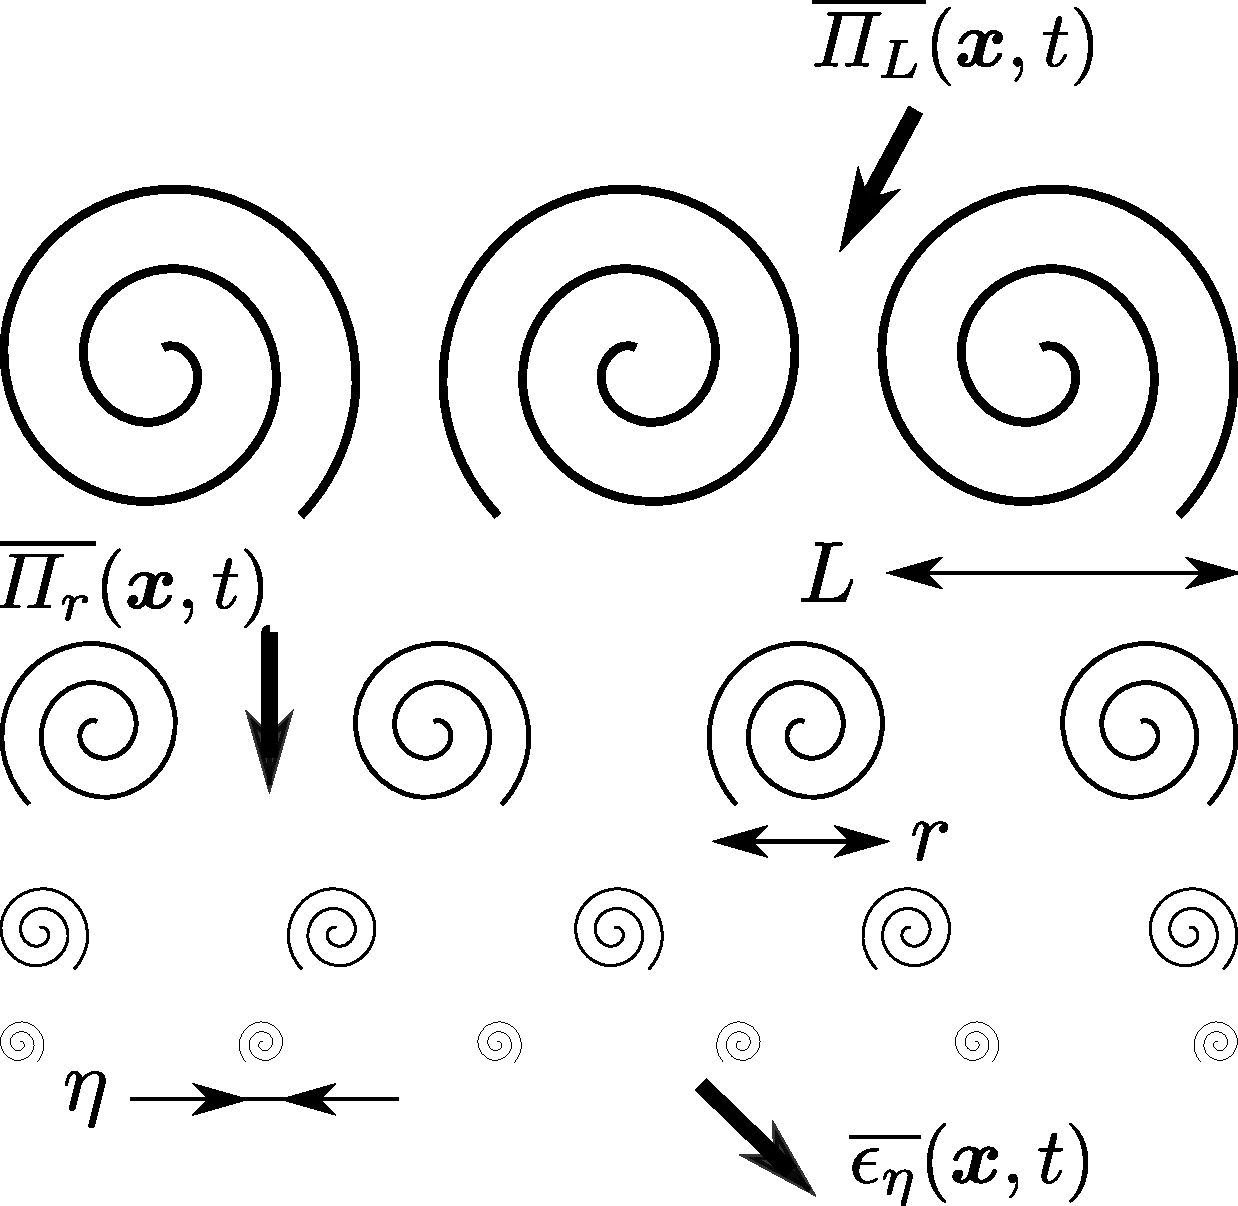
\includegraphics[bb=0.000000 0.000000 594.189270 578.870117, width=0.6\textwidth]{EnergyCascade_Schematic.pdf}
  \caption{
    エネルギカスケード描像の模式図.
    図の上部が大スケール渦,下部が小スケール渦を表し,エネルギが大スケールから小スケールに(上から下に)「カスケード」する様子を模式的に示している.}
  \label{fig:EnergyCascade_Schematic.pdf}
\end{figure}
この描像は,乱流をさまざまなスケールの渦を用いて説明する.
まず,境界条件や外力によって,マクロな長さスケール\(L\)程度の渦にエネルギが注入される.
エネルギを持った大スケール渦は,自身より小さな渦を生成しこれにエネルギを伝達する.
このエネルギ伝達が繰り返しおこなわれることで,エネルギが漸次より小さなスケールに「カスケード」する.
粘性が支配するスケール\(\eta\)程度の渦に伝達されたエネルギは,熱として散逸する.
エネルギカスケードは次節以降で述べるKolmogorovの乱流理論の骨子となる重要な描像である.
